\section{Theory}
\label{section: Theory}

\subsection{Electromigration}
Electromigration (EM) is the transport of material that takes place in a conductor under high enough current densities [1]. This causes voids and hillocks to appear in the conductor and, in the extreme case, a complete break will form in the conductor.

\begin{figure}[H]
	\centering
     \begin{subfigure}[b]{0.49\textwidth}
         \centering
         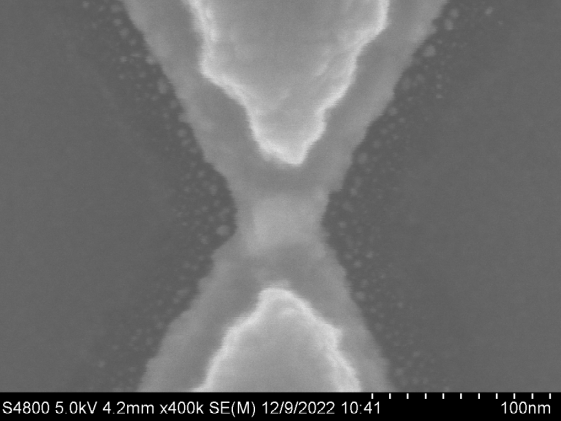
\includegraphics[width=\textwidth]{BeforeMigration.png}
         \caption{SEM image taken of a device before migration. \vspace{1.3cm}}
         \label{fig:BeforeMigration}
     \end{subfigure}
     \hfill
     \begin{subfigure}[b]{0.49\textwidth}
         \centering
         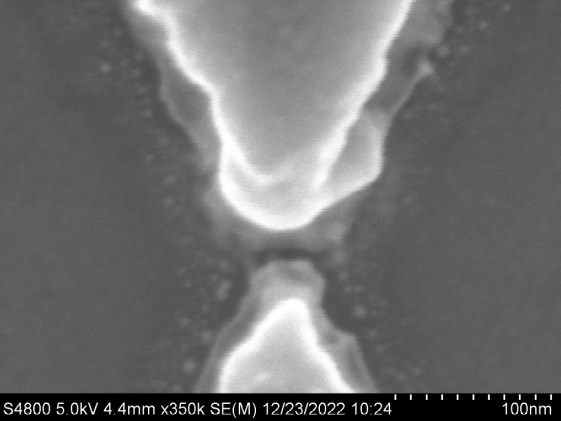
\includegraphics[width=\textwidth]{AfterMigration.png}
         \caption{SEM image taken of a device after migration. It is clear from the picture that material has moved from the bottom to the top in this image, against the direction of the applied bias voltage.}
         \label{fig:AfterMigration}
     \end{subfigure}
        \caption{Two SEM images taken before and after electromigration. The images are taken of different devices created with the same design. In the migration process, the bias voltage was applied from the bottom of the image towards the top. The regions of the device not shown in these images were not visibly changed during the migration process.}
        \label{fig:MigrationBeforeAfter}
        
\end{figure}

Historically, EM was of interest because it caused interconnects in integrated circuits to fail [1]. This was an expensive problem which received a lot of attention from the electronics industry. More recently, however, EM has also been used productively in creating nanoscale gaps in metallic structures. These gaps can have many uses, with the most prominent being single molecule junctions [1]. EM is useful for making single molecule junctions because the size of the gap that is created by EM is of the order of nanometers, the same order of magnitude as many molecules.

\subsubsection{Mechanisms}
The central mechanism driving EM is thermally activated diffusion of the atoms under forces resulting from bias voltage and current [1]. Atoms in the conductor are trapped in a potential well created by neighboring atoms. In order for an atom to escape the potential well, it either needs to be thermally excited such that its energy exceeds the height of the potential barrier, or the barrier must be lowered sufficiently by an applied force. The main forces acting on the atom when a voltage bias is applied to the conductor are the electron wind force, the direct force and the entropic diffusion force. 

When a bias voltage is applied to a conductor, the electrons of the conductor gain a non-zero average momentum. The electrons experience collisions with the atoms, in which momentum is transferred from the electrons to the atoms. When the electrons have non-zero average momentum, the average momentum imparted on the atoms is also non-zero. The electron wind force explains why, when imaging a conductor after EM has taken place, mass can normally be seen to have moved against the direction of the current.  

In a conductor, there are mobile electrons. As a result, the atoms become effectively ionic with a positive charge. When a voltage is applied across the conductor, the ions experience a Coulomb force in the direction of the bias voltage. This is the direct force, and it is directed in the opposite direction from the electron wind force, thus reducing the rate of atomic diffusion [1].

Whenever there exists a spatial concentration gradient, there will be a net movement of atoms in the direction opposite to this gradient, as described by the diffusion equation [1]. The result of this is that atoms located in regions of high atomic density experience a force pushing them in the direction of adjacent regions of lower atomic density. Since EM causes net flow of atoms in one direction, the region that atoms are moved to gets a higher atomic density, while the region that atoms are moved from gets a lower atomic density. This thus results in a concentration gradient pointed in the same direction as the mass flow, and therefore the entropic diffusion force will be pointed in the opposite direction. Entropic diffusion is therefore a stabilizing force which reduces the mass flux. 

Since thermally activated diffusion is the main mechanism behind EM, net mass flux in a conductor is more likely to start in a region of higher temperature. If the conductor has a spatially inhomogeneous thermal conductance coefficient, or experiences inhomogeneous Joule heating, this will cause some regions to become hotter than others, making EM more likely to occur in these regions. There are also regions in the conductor where the potential barrier experienced by the atoms is lower. Atoms on the surface of the conductor, and atoms placed next to grain boundaries, impurities and vacancies, all experience lower potential barriers. These sites are therefore also more likely places for EM to occur.

In order for EM to take place, the current density needs to be sufficiently high. This happens at some critical voltage $V_C$. 

\subsubsection{Effects of Size}
The size of the wire has a significant influence on electromigration. When the wire is of the order of tens of nanometers, as is the case in the devices studied in this thesis, EM tends to progress in a markedly different way as compared to macroscopic wires [1]. In nanoscale wires, the ratio of surface area to volume is orders of magnitude larger than it is, for example, in micron scale wires. In micron scale wires, atomic diffusion happens mainly along grain boundaries. In the smaller nanometric wires, however, diffusion along the surface of the wire dominates. In micron scale wires, macroscopic hillocks and voids tend to form. In nanowires, on the other hand, the wire experiences a gradual narrowing which is localized at the point of highest resistivity. This point experiences the strongest scattering and the highest amount of Joule heating, and therefore it experiences the highest amount of mass flux. The location of this point is dependent on the device geometry and on the microscopic details of the wire, such as the grain boundary structure. 

Studies investigating EM in nanowires have found that it takes place in stages. In the first stage, the wire gradually narrows in one place, with the rest of the wire remaining unchanged. In this stage, Joule heating of the wire causes surface atoms to be promoted to adatoms, which are then swept away against the direction of the current by the electron wind force. When the narrowing progresses to the point that transport becomes quasi-ballistic, the mechanism behind the EM changes. At this point, individual collisions between atoms and electrons are the main driver behind the transfer of mass [1]. 

\subsubsection{Controlling Electromigration}
When using EM to create useful nanogaps, it is important to have a high degree of control over the process. The size of the gap and the resistance of the junction need to be accurately controlled to tailor the junction to its application. When using the junction for single molecule transport measurements, for example, it is necessary that the gap size is similar to the size of the molecule. With regard to achieving this control, there are certain aspects of the device design and the procedure by which the voltage is applied that are particularly relevant. 

When creating a gap in a bridge using EM, the bias voltage will be applied not only over the bridge but also over other resistances between the bridge and the voltage source. The sum of those series resistances is denoted as $R_{S}$, while the resistance of the junction is denoted as $R_{J}$. The junction is the location in the bridge where migration takes place. $R_S$ is for example contributed to by the contact resistance of the voltage source and the resistance of any wires used to connect the voltage source to the junction. When $R_{S}$ is large compared to $R_{J}$, a constant or increasing voltage will cause heating in the junction, which will increase the EM in the junction. This further increases $R_J$, which in turn further increases the EM, in a positive feedback loop that causes a rapid and uncontrolled migration. This leads to an oversized gap and possibly the formation of islands of material inside the gap. In order to avoid this situation, the ratio of series resistance and junction resistance need to be kept in mind when designing the device. This is done for example by connecting the junction to large pads and wires, and making the bridge very thin or giving it a constricted design.

There are multiple ways in which the voltage can be applied to induce EM. Two straightforward ways are to simply ramp up the voltage until the wire breaks, or to apply a constant voltage which is higher than $V_C$ to the junction. These methods offer very little control over the final state of the junction after electromigration. In order to gain more control, the voltage can be applied in pulses. This process is known as pulse EM. Pulse migration adds the parameter of pulse duration, which can increase the level of control the operator has on the EM procedure. The way pulse EM can achieve a desired gap is by repeatedly applying pulses while measuring the resistance of the device. Once this resistance has reached the target resistance, no more pulses are applied. The height and width of the pulses can be changed by the operator based on the increase in resistance each pulse generates. While this method can work in practice [11], the level of control it affords tends to be lower than one can get when using feedback control, which we discuss next.

Feedback controlled EM (FCEM) is a process by which the applied voltage to the device is rapidly changed in response to changes in the resistance of the device [12]. This is done using software that controls the amount of bias voltage applied based on the corresponding amount of bias current. Measuring the current and updating the voltage happens with very high frequency. High frequency is required in order to be able to respond to the changes in the device resistance on an appropriate timescale, on the order of tens of kHz, such that voltage can be ramped back before the resistance has changed too much. The FCEM algorithm operates as follows. A human operator sets the target resistance $R_{Target}$ and the initial voltage $V_i$, and the maximal voltage $V_{max}$. The algorithm now starts to ramp the voltage in small increments from $V_i$ to $V_{max}$. For each applied bias voltage, the current is measured. Using the current, the resistance can be determined using the formula $R = V/I$. For the first few points of the ramp, the calculated resistance values are used to generate an average ramp resistance for the current ramp, $R_{Ramp}$. If, during the ramp, the measured resistance deviates from $R_{Ramp}$ by more than some threshold amount $c \cdot R_{Ramp}$, where $c$ is a parameter specified by the operator which is called the cut-off parameter, then the algorithm brings the current back to $V_i$. If the resistance at this point is still lower than $R_{Target}$, the algorithm starts a new ramp and a new iteration of the algorithm commences. By ramping the voltage back the migration is interrupted before the change in resistance has gotten very large. Because of this, the resistance can only increase in small increments, which allows FCEM to achieve a higher level of control regarding the final resistance. 

The values of the parameters specified by the operator need to be optimized to ensure that EM happens at a sufficient rate while still allowing the algorithm to ramp back fast enough to prevent sudden large changes in resistance [12]. In the first stage of migration, when transport is diffusive, migration happens smoothly and the resistance can be seen to go up gradually. In this stage, the operator should specify a low cutoff parameter. When migration halts or progresses too slowly, $V_{max}$ should be increased. In the second stage, where transport through the junction is ballistic, the migration happens more stochastically and the jumps in resistance are bigger. This stage starts roughly around the 1 k$\Omega$ resistance level, which corresponds to about a dozen atoms in most of the materials commonly used in EM. At this stage, the cut-off parameter should be set high, and the rate of migration controlled using $V_{max}$. The level of control the operator has over the resistance at this stage is lower. Once the resistance reaches a value of around one $R_\textrm{Q}$ = 12.9 k$\Omega$, the junction transitions to the tunnel regime and the level of control drops even further. At this point, the level of resistance reached is only partly controllable by the operator and trial and error on multiple devices may be needed to achieve the desired resistance.
\\

\noindent For certain metals at high enough temperatures, when EM is stopped after increasing the resistance past some threshold value, migration will continue without any applied voltage. This is known as self-breaking. Self breaking happens when atoms rearrange themselves in order to reduce their surface energy. Since the narrowed section of wire created through partial EM has a very large surface area compared to its volume, this is a very unfavored surface-energetic configuration. If the temperature is sufficient and the mobility of the atoms high enough, then the atoms will rearrange themselves in order to reduce their surface energy. In this process, atoms move away from the junction towards the bulk of the bridge. This is a gradual process, and it can be interrupted by cooling down the junction. This means that by stopping EM after the threshold has been reached, and then monitoring the resistance of the junction, the desired resistance can be reached by cooling down the junction once the resistance is close to the target. A benefit of self breaking is that in general the formation of metallic islands in the gap is rare when the gap is created through self breaking.


\subsection{Superconductivity and the Superconducting Proximity Effect}


Superconductivity is a phenomenon first discovered in Leiden in 1911 by Kamerlingh Onnes, when observed that the resistivity of mercury dropped to zero when it was cooled in liquid helium. Superconductivity is characterized by zero resistivity and a complete expulsion of magnetic field. Materials where superconductivity can occur are called superconductors. 

Superconductors are only superconducting when the temperature, current density and applied magnetic field are all low enough [13]. If these quantities become too large, a phase transition occurs and superconductance ceases. Figure \ref{fig:superconducting_phase_transition} shows a typical phase transition surface in temperature-current density-magnetic field space. The maximal temperature at which superconductivity can still occur is known as the critical temperature and is denoted $T_C$. Similarly, the maximal current density and magnetic field where superconductivity can still occur are called the critical current density and critical field, respectively, and are denoted by $J_C$ and $B_C$.

\begin{figure}[H]
     \centering
     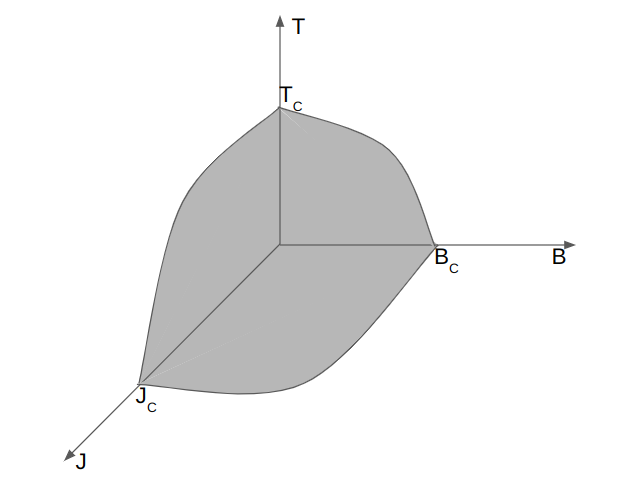
\includegraphics[width=\textwidth]{superconducting_phase_transition.png}
     \caption{A typical superconducting phase transition surface, depicted in gray.}
     \label{fig:superconducting_phase_transition}
        
\end{figure}


\subsubsection{Theoretical Frameworks}

Although superconductivity had been first discovered in 1911, it remained quite poorly understood until the revolutionary work done by Bardeen, Cooper and Schrieffer in 1957. The theory they set forth, the so called Bardeen-Cooper-Schrieffer (BCS) theory, is a microscopic theory that describes superconductivity in terms of phonon-mediated interactions between electrons [12]. In the theory, for superconductors at low enough temperatures, the electron-electron interaction becomes effectively attractive due to electron-phonon interactions. This causes electrons to pair up, forming pairs with opposite momentum and spin called Cooper pairs. The Cooper pairs all occupy the same macroscopic ground state. In the density of states, a gap opens up around the energy of this ground state. This gap is called the superconducting energy gap, and it has a magnitude $|\Delta|$. BCS theory predicts that at zero temperature, the energy gap is proportional to the critical temperature, according to the formula $|\Delta|$ = $1.764 k_BT_C$. \\


Another theory of superconductivity, which preceded BCS theory historically, is the Ginzburg-Landau (GL) theory [13]. GL theory provides a macroscopic, phenomenological description of superconductivity, in terms of a complex order parameter $\Delta$ = $|\Delta|e^{i\phi}$. It turns out that this order parameter is related to the wave function of the Cooper pair wave function. The magnitude of the order parameter is equal to the superconducting energy gap. The characteristic distance over which the order parameter shows significant variation is called the superconducting coherence length, and is denoted $\xi$. GL theory is valid close to $T_C$, when $|\Delta| << k_BT_C$. 

The Gor'kov theory of superconductivity is an extension of BCS theory that gives a description of the superconducting state in the framework of the Green's function formalism [13]. Gor'kov theory is able to predict the behavior of the order parameter and the density of states of the superconductor.

In the limit of $\lambda_F << \xi$, or, equivalently, $|\Delta| << E_F$, which is known as the quasi-classical limit, Gor'kov theory can be simplified. The resulting theory is known as the Eilenberger theory. If, additionally, a system is in the limit of strong disorder, i.e. when the mean free path $l << \xi$, the theory can be further simplified into the Usadel theory. The limit in which the Usadel theory is valid, is known as the "dirty" limit. Many of the results that can be derived using the Usadel theory are used throughout this work.



\iffalse 
Usadel describes superconductivity in terms of the complex functions $F$, which only depend on the so called "Matsubara frequency", $\hbar \omega = \pi k_BT(2n+1)$ and the position $\mathbf{r}$. The Usadel equations can be expressed in an especially simple form by introducing the variable $G = (1-FF^\ast)^{1/2}$. The Usadel equation for $F$ then becomes \cite{Likharev}

$$
2\omega F - D(\nabla - i \frac{2e}{\hbar c} \mathbf{A})\left[G\left(\nabla - i \frac{2e}{\hbar c} \mathbf{A}\right)F - F\nabla G \right] = 2 \hbar^{-1} \Delta G
$$

By summing $F$ with over the Matsubara frequencies, the measurable quantities, i.e. the supercurrent and order parameter, can be derived as follows:

$$
ln(T_C/T) = \Delta ln(T_C/T) = 2\pi k_BT \sum_{\omega > 0} [(\Delta / \hbar \omega) - F]
$$
and
$$
\mathbf{j_s} = \sigma_N(2\pi k_BT/e) \sum_{\omega > 0} Im[F^\ast \left(\nabla - i \frac{2e}{\hbar c} \mathbf{A}\right)F]
$$
\fi



\subsubsection{Proximity Effect and Andreev Reflections}
When a superconductor and a normal metal are brought into contact, there is a transition region in which the order parameter varies between its value deep inside the superconductor, $\Delta_{SC}$, and its value deep in the normal metal, which is 0. In this transition region, the normal metal has a nonzero order parameter and becomes superconducting. This is known as the superconducting proximity effect. The strength of the proximity effect decreases further away from the superconductor-normal metal (SN) interface, and the characteristic length over which this drop-off happens is denoted $\xi_N$, and is of the order of $\sqrt{D/T}$, where $D$ is the diffusion constant in the normal metal. Conversely, the order parameter inside the superconductor is lower closer to the interface with the normal metal than it is far away from this interface. As a result, superconductivity in this region is suppressed. This is called the inverse superconducting proximity effect. The proximity effect can be understood microscopically by examining the transport physics at an SN interface.
 

Charge transport at an SN interface happens in a way that is different from charge transport between two normal metals. If we assume that there is no tunnel barrier between the superconductor and normal metal, transport happens as follows; When an electron passes from the normal metal to the superconductor, and the energy $\varepsilon$ of the electron is higher than $|\Delta|$, the electron can enter the superconductor and occupy a single quasi-particle state. The density of states below $|\Delta|$ is zero, however, and therefore an electron coming from the normal metal with energy $\varepsilon < |\Delta|$ can not enter the superconductor in the normal way. In that case, a hole can be reflected from the SN interface at the same time the electron passes through, and in the process a Cooper pair added to the superconductor. This process is called Andreev reflection. Since a hole has charge e, and a Cooper pair has charge -2e, charge is conserved during Andreev reflection. In order to ensure conservation of energy, the hole needs to have energy -$\varepsilon$. Conversely, when charge is transported from the superconductor to the normal metal, the mechanism is reversed. If the charge crossing the SN barrier is a single quasi-particle with energy $\varepsilon > |\Delta|$ it can pass to the normal metal as it would when passing through a normal metal interface. When a Cooper pair is responsible for the charge transfer, two electrons enter the normal metal with an energy difference of $2\varepsilon$. These electrons still carry their Cooper pair correlation after passing the SN barrier. The characteristic time it takes the electrons to lose this correlation is the dephasing time $\tau = \hbar/\varepsilon$. In this time, the electrons travel a distance $L = \sqrt{D\tau}$ on average in the direction of propagation. As a result, the electrons with energy less than $D\hbar/L^2$ will still carry their Cooper pair correlations at distance L from the SN interface in the direction of propagation. When $L$ is the total length of the normal metal, this energy is called the Thouless energy, and denoted $E_{Th}$.

\begin{equation}
\label{eq:E_Th(D,L)}
E_{Th} = D\hbar/L^2
\end{equation}



 Since the electrons with $\varepsilon > |\Delta|$ are coming from the single particle continuum and did not carry Cooper pair correlation to begin with, those electrons in the normal metal that carry Cooper pair correlations must have energy $\varepsilon < \mathrm{min}\left(E_{Th}, |\Delta|\right)$, and only those electrons contribute to the superconducting transport through the normal metal.


\subsubsection{Superconductivity in SN Bilayers}
In situations where the Usadel theory is valid, the critical temperature of an SN bilayer can be predicted theoretically based on the Usadel formalism, as is done in [15] for example for the case of thin films. In this case, the thin film limit is that limit where the thickness of the superconductor and of the normal metal are small in comparison to their respective superconducting coherence lengths. The formula derived for the critical temperature $T_C$ of an SN bilayer in this limit is given by eq. \ref{eq:BilayerTc}.

\begin{equation}
\label{eq:BilayerTc}
T_C = T_{C0} \left[ \frac{d_s}{d_0} \frac{1}{1.13(1+1/\alpha)} \frac{1}{t} \right] ^\alpha
\end{equation}

\noindent where $$ 1/d_0 = (\pi/2)k_BT_{C0}\lambda_f^2n_s $$ and $$ \alpha = d_nn_n/d_sn_s $$ In these equations, $T_{C0}$ is the critical temperature of the bare superconductor, $d_n$ and $d_s$ are the thicknesses of the normal metal and superconductor, respectively, and $n_n$ and $n_s$ are the respective volumetric electron density of states at the Fermi energy. The parameter $t$ represents the interface transparency. In practice, for most clean metals and interfaces, $t$ tends to be of the order of 0.1 to 1. The interface parameter can be reduced in case of a lattice mismatch, a difference in Fermi velocity, or a contaminated or oxidized contact surface.\\

The devices studied in this thesis contain Pd-Nb and Au-Nb bilayers. Therefore, these materials are of particular interest, and for this reason those material properties that occur in equation \ref{eq:BilayerTc} have been tabulated in table \ref{tab:Bilayer_Table}.

\begin{table}[H]
\centering
\caption{Critical temperature $T_{C0}$ and volumetric electron density of states at the Fermi level $n$ for relevant materials.}
\label{tab:Bilayer_Table}
\begin{tabular}{|c|c|c|}

\hline 
Metal & $T_{C0}$ (K) & $n$ (states / eVcm$^3$) \\ 
\hline 
Nb, 100 nm & 9.1  & 5.07 $\cdot$ 10 $^{22}$ \\ 
\hline 
Nb, 50 nm & 8.9 & 5.07 $\cdot$ 10 $^{22}$ \\ 
\hline 
Ti & 0.49  & 2.93 $\cdot$ 10 $^{22}$ \\ 
\hline 
Pd & - & 1.55 $\cdot$ 10 $^{23}$ \\ 
\hline 
Au & - & 1.60 $\cdot$ 10 $^{22}$ \\ 
\hline 
\end{tabular} 
\end{table}

Once the value of $T_C$ is known, the energy gap of the bilayer can be calculated simply using $\Delta = 1.764 k_BT_C$ in the case of a BCS superconductor.



\subsubsection{Charge Transport in Weak Links}

In the literature on superconductivity, the term "weak link" refers to any structure that connects two bulk superconducting electrodes, for which the critical current is much less than the critical current of the electrodes. All the devices studied in this thesis have this structure, and the theory of weak links is therefore of particular interest.\\


There are several parameters which characterize a weak link. The distance between the superconducting electrodes is referred to as the length $L$ of the weak link. There is another length scale that plays a more central role in weak link transport, however, and that is the effective length $L_\mathrm{eff} \geq L$. The effective length is the length scale over which nonlinear effects are localized. In general, the nonlinear effects are localized over shorter distances in weak links with lower conductivity. Weak links for which the superconducting coherence length $\xi$ is much greater than $L_\mathrm{eff}$ are classified as short junctions, and those for which $\xi \lesssim L_\mathrm{eff}$ are classified as long junctions. 

Within the short junction limit, there is a second classification which is based on the electron mean free path $l$. Weak links for which the effective length is much greater than $l$ are classified as "dirty", and those in the opposite limit are classified as "clean". Usually, electrons in a weak link experience diffusive scattering on the film surface, and as a result $l$ tends to be of the order of the film thickness which is much less than $L_\mathrm{eff}$. 


The devices studied in this thesis have bridge thickness that is much smaller than the bridge length and therefore also much smaller than the effective length, and they can thus be classified as dirty weak links.


\subsubsection{Josephson Junctions and the $I_CR_N$ Product}

The critical $I_C$ is defined as the maximal equilibrium supercurrent of a system [14]. When the current crosses $I_C$, there is a jump in the resistance of the system. The magnitude of this jump is the normal resistance $R_N$. Together, the critical current and normal resistance define a voltage, the critical voltage $V_C = I_CR_N$. The critical voltage is an important parameter in the description of many superconducting systems.

In the case of superconductor-insulator-superconductor (S-I-S) junctions, the critical voltage is proportional to the energy gap:

$$
I_CR_C = \pi \Delta/ 2e
$$


For the special case of dirty S-N-S junctions, the Usadel equations can be solved to find the relationship between $V_C$ and temperature for various ratios of $L$ and $\xi_N$ at the critical temperature of the superconductor. This relationship is captured in the graph in figure \ref{fig:V_C_of_T_for_different_L_over_Xi}, which has been reproduced from [13] with slight modifications. 

\begin{figure}[H]
     \centering
     \hspace{0.7cm}
     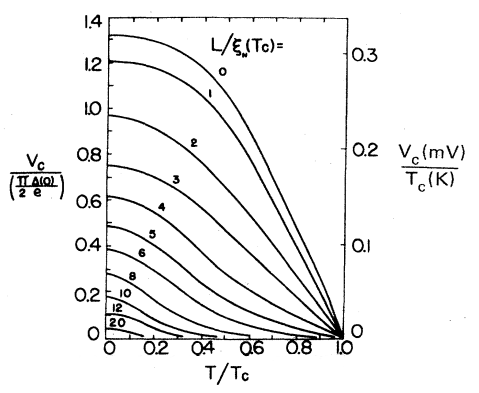
\includegraphics[width=0.5\textwidth]{Likharev_Graph.png}
     \caption{This figure has been reproduced with modifications from [13]. Theoretical predictions of the critical voltage $V_C$ as a function of temperature, for different values of $L/\xi_N(T_C)$.}
     \label{fig:V_C_of_T_for_different_L_over_Xi}
        
\end{figure}

In this limit, the Usadel equations also allow for the derivation of formula \ref{eq:Xi_N_of_T}. In this formula, $D$ is the diffusion coefficient in the normal metal. 


\begin{equation}
\label{eq:Xi_N_of_T}
\xi_N(T) = \sqrt{\frac{\hbar D}{2\pi k_BT}}
\end{equation}







\iffalse
In long junctions in the dirty limit, the Thouless energy and $I_CR_N$ are found to be proportional at zero temperature:

\begin{equation}
\label{eq:IcRn_at_low_T}
eI_CR_N = \pi E_{Th} 
\end{equation}


This equation can be extended using quasiclassical theory when $E_{Th} << \Delta$, and the extended relationship is given in equation \ref{eq:generalized_thouless_energy}.

\begin{equation}
\label{eq:generalized_thouless_energy}
eI_CR_N \approx \frac{32}{3+2\sqrt{2}} E_{Th} \left[ \frac{2\pi T}{E_{Th}} \right]^{\frac{3}{2}}e^{-\sqrt{\frac{2\pi T}{E_{Th}}}}
\end{equation}


Get the following formula in somewhere :

$$
D = v_f l/3
$$


Length and effective length, Long and Short junction limit, Dirty vs Clean limit of junction (n.b. not of superconductor)


Gindsberg landau assumptions + formulas

Formula 41 on IcRn product and $\Delta_{1/2}$

Usadel equations assumptions + formulas

Formula 76, 78 on IcRn

Formula 142 maybe?

\fi




